%%%%%%%%%%%%%%%%%%%%%%%%%%%%%%%%%%%%%%%%%
% Beamer Presentation
% LaTeX Template
% Version 2.0 (March 8, 2022)
%
% This template originates from:
% https://www.LaTeXTemplates.com
%
% Author:
% Vel (vel@latextemplates.com)
%
% License:
% CC BY-NC-SA 4.0 (https://creativecommons.org/licenses/by-nc-sa/4.0/)
%
%%%%%%%%%%%%%%%%%%%%%%%%%%%%%%%%%%%%%%%%%

%----------------------------------------------------------------------------------------
%	PACKAGES AND OTHER DOCUMENT CONFIGURATIONS
%----------------------------------------------------------------------------------------

\documentclass[
	11pt, % Set the default font size, options include: 8pt, 9pt, 10pt, 11pt, 12pt, 14pt, 17pt, 20pt
	%t, % Uncomment to vertically align all slide content to the top of the slide, rather than the default centered
	%aspectratio=169, % Uncomment to set the aspect ratio to a 16:9 ratio which matches the aspect ratio of 1080p and 4K screens and projectors
]{beamer}

\graphicspath{{images/}{./}} % Specifies where to look for included images (trailing slash required)

\usepackage{booktabs} % Allows the use of \toprule, \midrule and \bottomrule for better rules in tables

%----------------------------------------------------------------------------------------
%	SELECT LAYOUT THEME
%----------------------------------------------------------------------------------------

% Beamer comes with a number of default layout themes which change the colors and layouts of slides. Below is a list of all themes available, uncomment each in turn to see what they look like.

%\usetheme{default}
%\usetheme{AnnArbor}
%\usetheme{Antibes}
%\usetheme{Bergen}
%\usetheme{Berkeley}
%\usetheme{Berlin}
%\usetheme{Boadilla}
%\usetheme{CambridgeUS}
%\usetheme{Copenhagen}
%\usetheme{Darmstadt}
%\usetheme{Dresden}
%\usetheme{Frankfurt}
%\usetheme{Goettingen}
%\usetheme{Hannover}
%\usetheme{Ilmenau}
%\usetheme{JuanLesPins}
%\usetheme{Luebeck}
\usetheme{Madrid}
%\usetheme{Malmoe}
%\usetheme{Marburg}
%\usetheme{Montpellier}
%\usetheme{PaloAlto}
%\usetheme{Pittsburgh}
%\usetheme{Rochester}
%\usetheme{Singapore}
%\usetheme{Szeged}
%\usetheme{Warsaw}

%----------------------------------------------------------------------------------------
%	SELECT COLOR THEME
%----------------------------------------------------------------------------------------

% Beamer comes with a number of color themes that can be applied to any layout theme to change its colors. Uncomment each of these in turn to see how they change the colors of your selected layout theme.

%\usecolortheme{albatross}
\usecolortheme{beaver}
% \usecolortheme{beetle}
% \usecolortheme{crane}
% \usecolortheme{dolphin}
% \usecolortheme{dove}
% \usecolortheme{fly}
% \usecolortheme{lily}
% \usecolortheme{monarca}
% \usecolortheme{seagull}
%\usecolortheme{seahorse}
%\usecolortheme{spruce}
%\usecolortheme{whale}
%\usecolortheme{wolverine}

%----------------------------------------------------------------------------------------
%	SELECT FONT THEME & FONTS
%----------------------------------------------------------------------------------------

% Beamer comes with several font themes to easily change the fonts used in various parts of the presentation. Review the comments beside each one to decide if you would like to use it. Note that additional options can be specified for several of these font themes, consult the beamer documentation for more information.

\usefonttheme{default} % Typeset using the default sans serif font
%\usefonttheme{serif} % Typeset using the default serif font (make sure a sans font isn't being set as the default font if you use this option!)
%\usefonttheme{structurebold} % Typeset important structure text (titles, headlines, footlines, sidebar, etc) in bold
%\usefonttheme{structureitalicserif} % Typeset important structure text (titles, headlines, footlines, sidebar, etc) in italic serif
%\usefonttheme{structuresmallcapsserif} % Typeset important structure text (titles, headlines, footlines, sidebar, etc) in small caps serif

%------------------------------------------------

%\usepackage{mathptmx} % Use the Times font for serif text
\usepackage{palatino} % Use the Palatino font for serif text

%\usepackage{helvet} % Use the Helvetica font for sans serif text
\usepackage[default]{opensans} % Use the Open Sans font for sans serif text
%\usepackage[default]{FiraSans} % Use the Fira Sans font for sans serif text
%\usepackage[default]{lato} % Use the Lato font for sans serif text

%----------------------------------------------------------------------------------------
%	SELECT INNER THEME
%----------------------------------------------------------------------------------------

% Inner themes change the styling of internal slide elements, for example: bullet points, blocks, bibliography entries, title pages, theorems, etc. Uncomment each theme in turn to see what changes it makes to your presentation.

%\useinnertheme{default}
\useinnertheme{circles}
%\useinnertheme{rectangles}
%\useinnertheme{rounded}
%\useinnertheme{inmargin}

%----------------------------------------------------------------------------------------
%	SELECT OUTER THEME
%----------------------------------------------------------------------------------------

% Outer themes change the overall layout of slides, such as: header and footer lines, sidebars and slide titles. Uncomment each theme in turn to see what changes it makes to your presentation.

%\useoutertheme{default}
%\useoutertheme{infolines}
%\useoutertheme{miniframes}
%\useoutertheme{smoothbars}
%\useoutertheme{sidebar}
%\useoutertheme{split}
%\useoutertheme{shadow}
%\useoutertheme{tree}
%\useoutertheme{smoothtree}

%\setbeamertemplate{footline} % Uncomment this line to remove the footer line in all slides
%\setbeamertemplate{footline}[page number] % Uncomment this line to replace the footer line in all slides with a simple slide count

%\setbeamertemplate{navigation symbols}{} % Uncomment this line to remove the navigation symbols from the bottom of all slides

%----------------------------------------------------------------------------------------
%	PRESENTATION INFORMATION
%----------------------------------------------------------------------------------------

\title[Kazooformation]{Kazooformation} % The short title in the optional parameter appears at the bottom of every slide, the full title in the main parameter is only on the title page

\subtitle{Bluring the lines between what is possible and what is reasonable} % Presentation subtitle, remove this command if a subtitle isn't required

\author[Joshua Jerred]{Joshua Jerred} % Presenter name(s), the optional parameter can contain a shortened version to appear on the bottom of every slide, while the main parameter will appear on the title slide

\institute[UT]{Utah Tech} % Your institution, the optional parameter can be used for the institution shorthand and will appear on the bottom of every slide after author names, while the required parameter is used on the title slide and can include your email address or additional information on separate lines

\date[\today]{} % Presentation date or conference/meeting name, the optional parameter can contain a shortened version to appear on the bottom of every slide, while the required parameter value is output to the title slide

%----------------------------------------------------------------------------------------

\begin{document}

\begin{frame}
  % \frametitle{test}

  \begin{itemize}
    \item Wi-Fi: Quadrature Amplitude Modulation
    \item Bluetooth: Gaussian Frequency Shift Keying
    \item 5G: Orthogonal Frequency Division Multiplexing
    \item Broadcast TV: 8-level Vestigial Sideband Modulation
  \end{itemize}

  \begin{figure}
    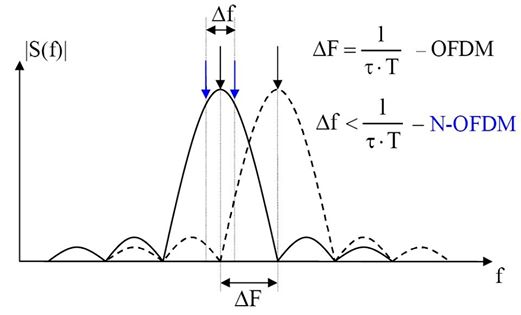
\includegraphics[width=0.6\linewidth]{ofdm.png}
    \caption{Subcarriers system of OFDM signals after FFT (Wikipedia)}
  \end{figure}

\end{frame}

%----------------------------------------------------------------------------------------
%	TITLE SLIDE
%----------------------------------------------------------------------------------------

\begin{frame}
  \titlepage % Output the title slide, automatically created using the text entered in the PRESENTATION INFORMATION block above
\end{frame}

%----------------------------------------------------------------------------------------
%	PRESENTATION BODY SLIDES
%----------------------------------------------------------------------------------------

\section{Intro} % Sections are added in order to organize your presentation into discrete blocks, all sections and subsections are automatically output to the table of contents as an overview of the talk but NOT output in the presentation as separate slides

%------------------------------------------------

\begin{frame}
  \frametitle{The New Physical Layer}

  \begin{columns}[c] % The "c" option specifies centered vertical alignment while the "t" option is used for top vertical alignment
    \begin{column}{0.7\textwidth} % Left column width
      % Assumptions:
      % \begin{itemize}
        % \item DSP and information theory are inherently boring topics
        % \item Kazoos are not boring
      % \end{itemize}
      \begin{center}
        % 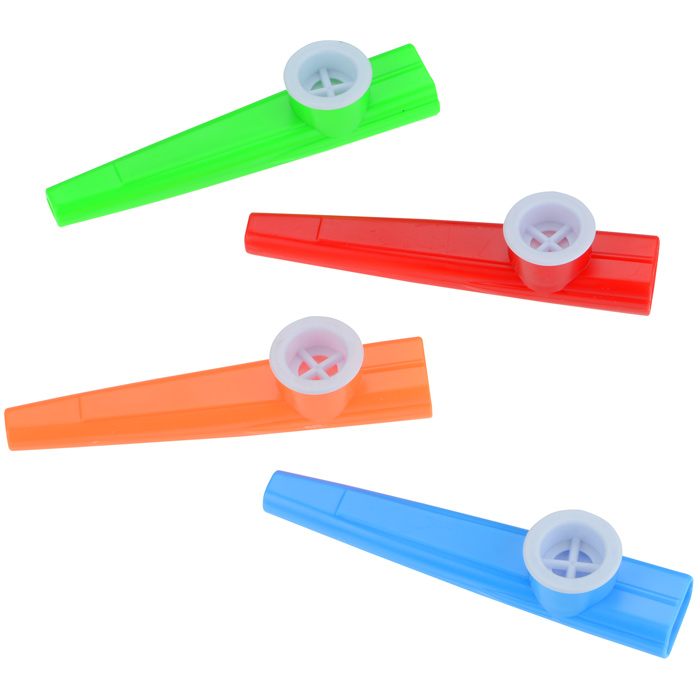
\includegraphics[width=0.6\linewidth]{kazoos.png}
        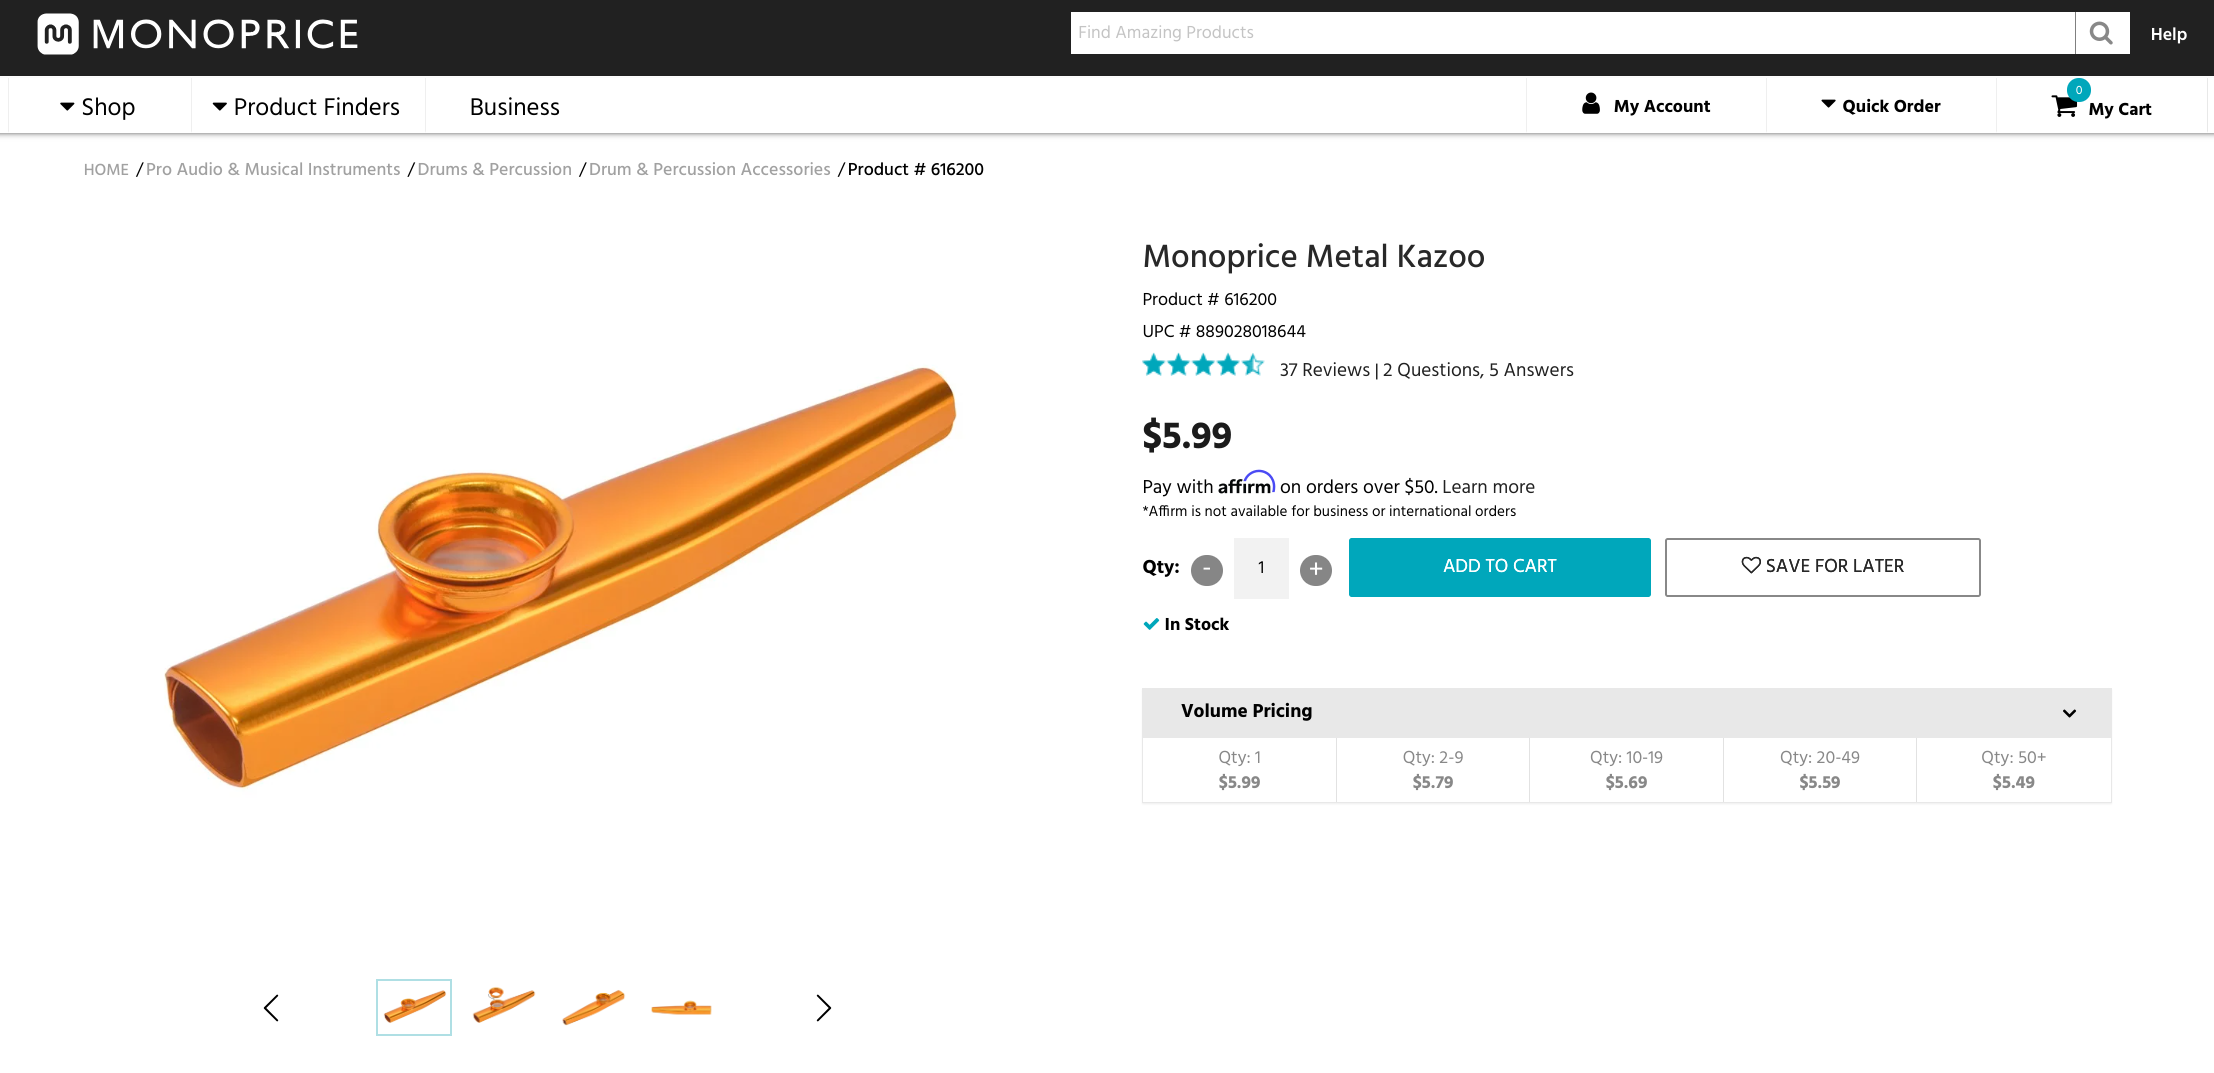
\includegraphics[width=1\linewidth]{monoprice.png}
      \end{center}
    \end{column}
    \begin{column}{0.25\textwidth} % Right column width
      \begin{center}
        \begin{figure}
          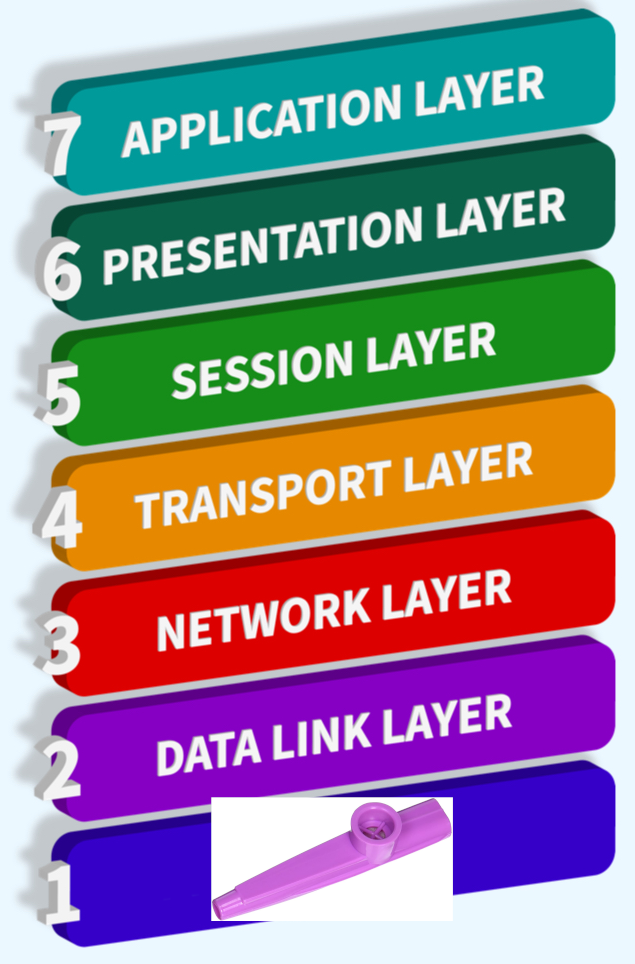
\includegraphics[width=1\linewidth]{new_osi_model.png}
        \end{figure}
      \end{center}
    \end{column}
  \end{columns}

\end{frame}

%------------------------------------------------

\begin{frame}
  % \frametitle{The New Physical Layer}

  A series of discrete kazoo signals

  \begin{center}
    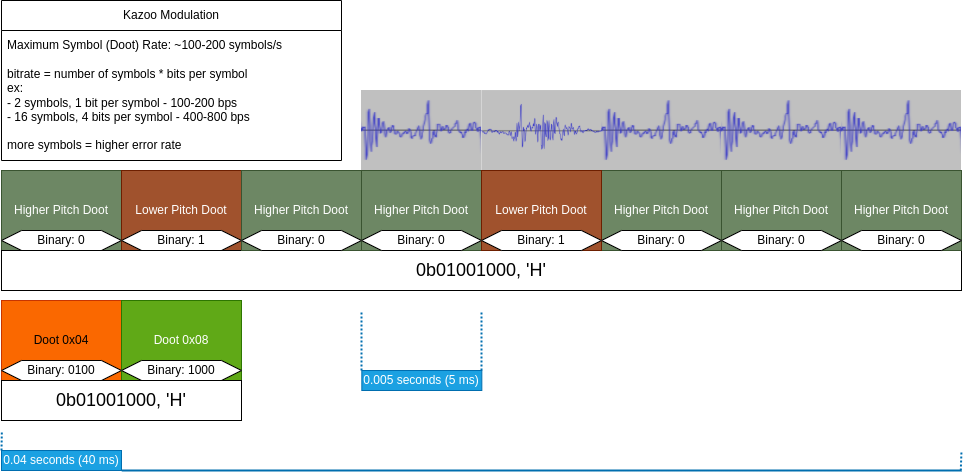
\includegraphics[width=1\linewidth]{kazoo_signals.png}
  \end{center}


\end{frame}

%------------------------------------------------

% \begin{frame}
  % \frametitle{Project Features}
% 
  % \begin{center}
    % 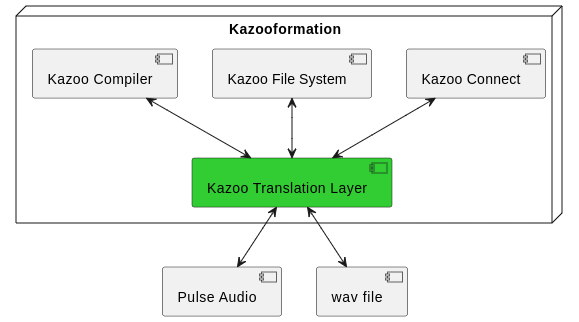
\includegraphics[width=0.6\linewidth]{org_diagram.png}
  % \end{center}
% \end{frame}

%------------------------------------------------

% \begin{frame}
  % \frametitle{Implementation Realities}

  % \begin{center}
    % 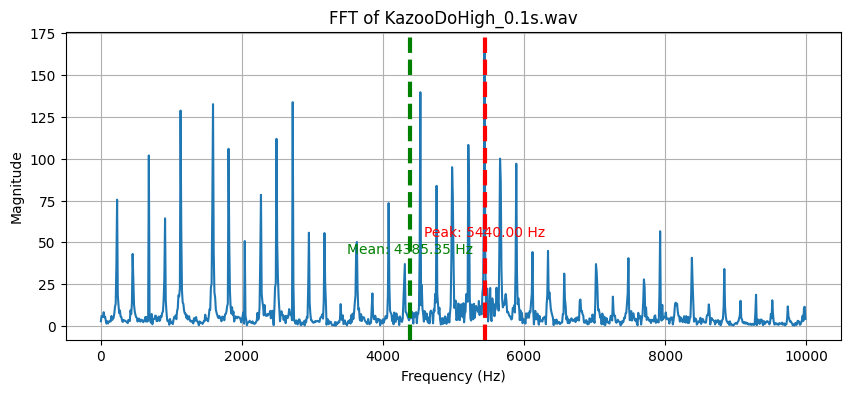
\includegraphics[width=1\linewidth]{fft_1.png}
  % \end{center}

  % \bigskip % Vertical whitespace

  % \begin{enumerate}
  %   \item Real time telemetry data and specific data upon request
  %   \item Remote control of systems and sensors
  %   \item Early flight termination
  %   \item Flight path control with ground based winds aloft data and controlled ballast release / gas venting
  %   \item Human intervention after launch when things go wrong
  % \end{enumerate}
% \end{frame}

%------------------------------------------------

% \begin{frame}
  % \frametitle{Technical Resources Used}
  % \begin{enumerate}
    % \item C++20 w/CMake and GTest (Heavily Reliant on Unit Tests)
    % \item FFTW3 (C++ FFT Lib) \& Pulse Audio (Audio Input/Output)
    % \item Numpy, Pandas, and Matplotlib for FFT visualization
  % \end{enumerate}
% \end{frame}

%-------------------------------------------------------------------------------

\begin{frame}
  \frametitle{Commercial \& Governmental Applications}
  JTRS: Hardware that supports unspecified and ever changing modulation/demodulation software
  
  \begin{columns}[c] % The "c" option specifies centered vertical alignment while the "t" option is used for top vertical alignment
    \begin{column}{0.4\textwidth} % Left column width
      \begin{center}
        
\includegraphics[width=1\linewidth]{jtrs_badge.jpeg}
      \end{center}
    \end{column}
    \begin{column}{0.7\textwidth} % Right column width
      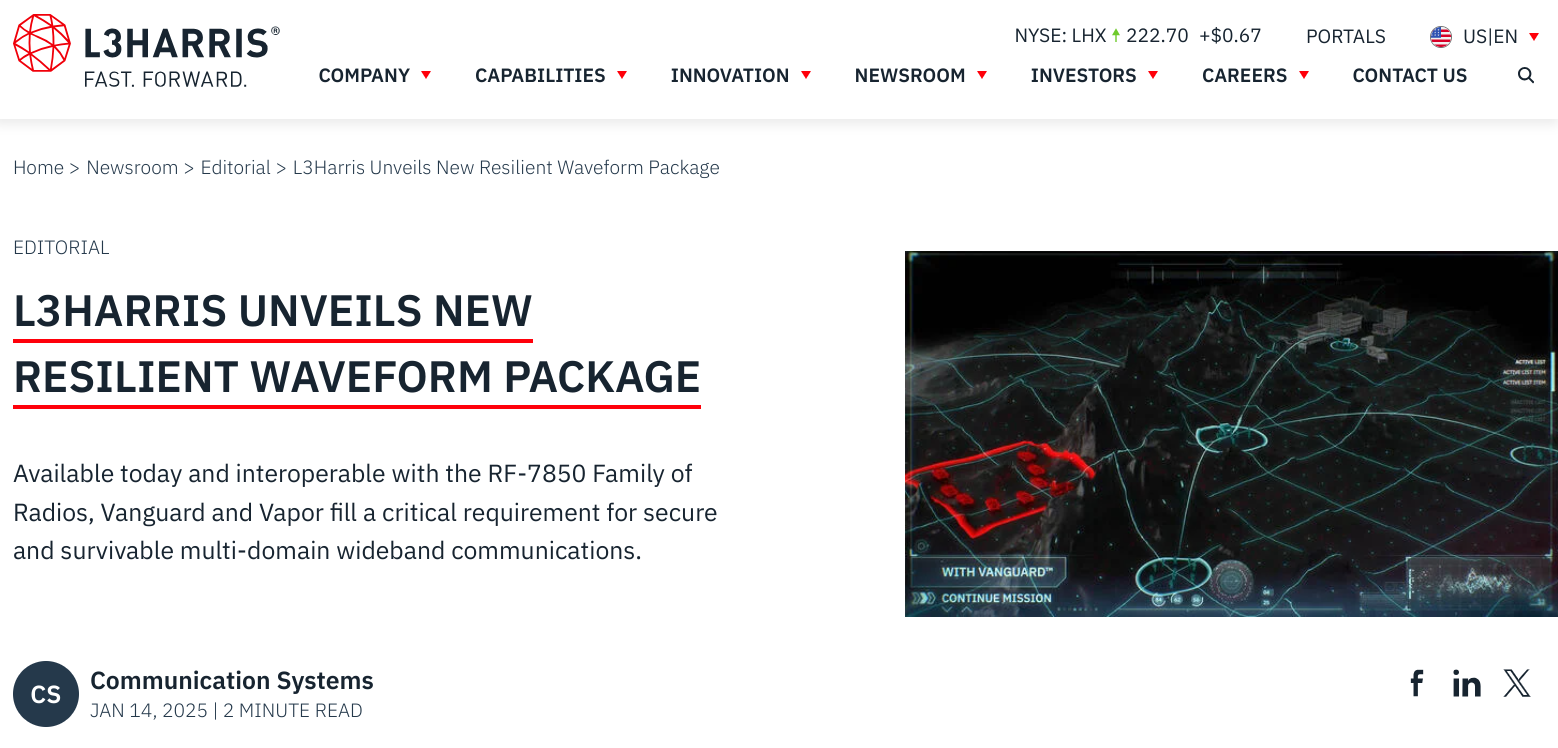
\includegraphics[width=1\linewidth]{l3harris.png}
      \begin{center}
      \end{center}
    \end{column}
  \end{columns}
\end{frame}

%-------------------------------------------------------------------------------

\end{document}